\documentclass{warpdoc}
\newlength\lengthfigure                  % declare a figure width unit
\setlength\lengthfigure{0.158\textwidth} % make the figure width unit scale with the textwidth
\usepackage{psfrag}         % use it to substitute a string in a eps figure
\usepackage{subfigure}
\usepackage{rotating}
\usepackage{pstricks}
\usepackage[innercaption]{sidecap} % the cute space-saving side captions
\usepackage{scalefnt}
\usepackage{amsbsy}
\usepackage{bm}
\usepackage{amsmath}

%%%%%%%%%%%%%=--NEW COMMANDS BEGINS--=%%%%%%%%%%%%%%%%%%%%%%%%%%%%%%%%%%
\newcommand{\alb}{\vspace{0.2cm}\\} % array line break
\newcommand{\mfd}{\displaystyle}
\renewcommand{\fontsizetable}{\footnotesize\scalefont{0.7}}
\renewcommand{\fontsizefigure}{\footnotesize}
\newcommand{\Bdipole}{B_{\rm d}}
\newcommand{\ns}{{n_{\rm s}}}
\newcommand\frameeqn[1]{\fbox{$\displaystyle #1$}}
\newcommand\framealign[1]{\fbox{\begin{align}#1\end{align}}}
\newcommand{\nd}{3}

\renewcommand{\vec}[1]{\bm{#1}}

\setcounter{tocdepth}{3}
\let\citen\cite

%%%%%%%%%%%%%=--NEW COMMANDS BEGINS--=%%%%%%%%%%%%%%%%%%%%%%%%%%%%%%%%%%

\setcounter{tocdepth}{3}

%%%%%%%%%%%%%=--NEW COMMANDS ENDS--=%%%%%%%%%%%%%%%%%%%%%%%%%%%%%%%%%%%%



\author{
  Bernard Parent
}

\email{
  bernparent@gmail.com
}

\department{
  Dept.\ of Aerospace Engineering
}

\institution{
  Pusan National University
}

\title{
  Electromagnetic Fields Module  
}

\date{
  2015
}

%\setlength\nomenclaturelabelwidth{0.13\hsize}  % optional, default is 0.03\hsize
%\setlength\nomenclaturecolumnsep{0.09\hsize}  % optional, default is 0.06\hsize

\nomenclature{

  \begin{nomenclaturelist}{Roman symbols}
   \item[$a$] speed of sound
  \end{nomenclaturelist}
}


\abstract{
abstract
}

\begin{document}
  \pagestyle{headings}
  \pagenumbering{arabic}
  \setcounter{page}{1}
%%  \maketitle
  \makewarpdoctitle
%  \makeabstract
  \tableofcontents
%  \makenomenclature
%%  \listoftables
%%  \listoffigures




\section{Charged Species Momentum Conservation Equation}


We here derive the drift-diffusion model of the momentum equation following Parent \cite{jcp:2011:parent}.  First, denoting a particular species with the subscript/superscript $k$, the inviscid form of the momentum equation can be written as:
%
\begin{equation}
  m_{k} N_k \frac{{\partial} \vec{V}^k}{\partial t} 
  +m_{k} N_k \vec{V}^k \cdot \vec{\nabla} \vec{V}^k 
  =
  C_k N_k (\vec{E}+\vec{V}^k\times \vec{B})-\frac{|C_k|N_k}{\mu_k} \left( \vec{V}^k -\vec{V}^{\rm n} \right) -\vec{\nabla} P_k
\end{equation}
%
with $m_k$ the mass of the ion or electron, $C_k$ is the charge of the ion or electron under consideration (equal to $-e$ for the electrons, $+e$ for the singly-charged positive ions, $-e$ for the singly-charged negative ions, $-2e$ for the doubly-charged negative ions, etc.), $\vec{V}^k$ the species velocity (including drift and diffusion), $\vec{V}^{\rm n}$ the velocity of the neutrals, $\mu_k$ the species mobility, $N_k$ the species number density, $\vec{\nabla} P_k$ the pressure gradient vector of the species under consideration,  $\vec{E}$  the electric field vector, and $\vec{B}$ the magnetic field vector. 


In the latter, the forces originating from the shear stresses and from the collisions between charged species are assumed to be negligible compared to the forces originating from the collisions of the charged species with the neutrals. The latter are good assumptions for a weakly-ionized gas. Indeed, should the ionization fraction be less than $10^{-4}$, it can be shown that the force due to collisions between charged species would amount to less than 1\% of the force induced by ion-neutral or electron-neutral collisions, and that the force resulting from the shear stresses would typically amount to an even smaller quantity.


It is noted that the terms including the pressure gradients are retained. Indeed, it can  be shown that the change in momentum due to the ion and electron pressure gradients is not always negligible for weakly-ionized gases. For instance, not only do the charged species pressure gradients become substantial within the cathode sheaths, but the pressure gradients can also be of importance in the vicinity of shockwaves and in regions with low gas density. 

Nonetheless, it can be shown that the forces due to pressure gradients are unlikely to exceed significantly the electromagnetic forces for typical flowfields. Then, taking this into consideration, a simple derivation shows that the change in inertia of the electrons can be assumed negligible as long as the following restrictions are met: 
%
\begin{equation}
T_{\rm e} < 60,000 ~{\rm K}
\end{equation}   
%
and
%
\begin{equation}
\left| \frac{1}{P_{\rm e}} \nabla P_{\rm e}\right| \ll \frac{|C_{\rm e}|}{\mu_{\rm e} \sqrt{ m_{\rm e}  k_{\rm B} T_{\rm e}}} 
\end{equation}   
%
with $T_{\rm e}$ the electron temperature, $m_{\rm e}$ the mass of the electron, and $k_{\rm B}$ the Boltzmann constant. The restriction on the electron temperature is easily satisfied in most weakly-ionized airflow problems. Indeed, even under very high electromagnetic fields, the electron temperature rarely exceeds 30,000~K. As for the restriction on the gradient of the electron pressure gradient, it would become invalid only if the electron pressure varies abruptly over a distance of less than one micrometer (in sea-level air). This is unlikely to occur due to the strong electron diffusion effectively prohibiting any such sudden change in the electron properties.   

Further, it can be proven that the change in inertia of the ions can be assumed negligible compared to the ion pressure gradient as long as
%
\begin{equation}
 \frac{\vec{|\vec{E^{\rm i}}|}}{N} \ll  \left(\frac{k_{\rm B} T^2}{T_{\rm ref} N_{\rm ref}^2 m_{\rm i}     (\mu_{\rm i})^2_{\rm ref}}\right)^\frac{1}{2}
\label{eqn:ioninertianegligible_condition1}
\end{equation}
%
Alternately, the change in ion inertia can be assumed negligible compared to the electric field force if the following is true
%
\begin{equation}
 \frac{ |N_{\rm i}-N_{\rm e}|}{N} \ll \frac{\epsilon_0}{m_{\rm i} (\mu_{\rm i})^2_{\rm ref}N_{\rm ref}}
\frac{P}{P_{\rm ref}}
\label{eqn:ioninertianegligible_condition2}
\end{equation}
%
with $\vec{E^{\rm i}}$ the electric field in the ion frame of reference, $N$ the number density of the bulk of the plasma, $m_{\rm i}$ the mass of the ion, $\epsilon_0$ the permittivity of free space, $P$ the pressure of the bulk of the gas, and $(\mu_{\rm i})_{\rm ref}$ the ion mobility evaluated at a reference temperature $T_{\rm ref}$, at a reference pressure $P_{\rm ref}$ and at a reference number density $N_{\rm ref}$. Because both the pressure gradient and electric field terms are kept in the momentum equation, only one of the above two conditions needs to be met for the ion inertia to be considered negligible. Then, from Eqs.\ (\ref{eqn:ioninertianegligible_condition1}) and (\ref{eqn:ioninertianegligible_condition2}), it can be easily deduced that for air plasmas at a pressure varying between 0.01 and 1~atm, the change in inertia of the ion $\rm N_2^+$ would become of importance only when three conditions are found conjunctly: (i) the reduced electric field is in the order of $10^{-19}$~V~m$^2$ or more, and (ii) the plasma has significant non-neutrality, and (iii) the ionization fraction is more than  $10^{-6}$--$10^{-4}$. Except perhaps in the cathode sheath, such is unlikely to occur for weakly-ionized airflow.   

Thus, after assuming that the inertia change is negligible and that  the momentum loss or gain through collisions between charged species is negligible, the momentum equation becomes \cite{jcp:2011:parent}: 
%
\begin{equation}
\frameeqn{
  \vec{V}^k=\vec{V}^{\rm n} + s_k \mu_k \left(\vec{E}+\vec{V}^k \times \vec{B}\right)-\frac{\mu_k}{|C_k| N_k}\nabla P_k
}
 \label{eqn:Vvector}
\end{equation}
% 
Then, after regrouping all $\vec{V}^k-\vec{V}^{\rm n}$ terms on the LHS the momentum equation in vector form becomes:
%
\begin{equation}
  \vec{V}^{k}-\vec{V}^{\rm n}- s_k \mu_k(\vec{V}^{k}-\vec{V}^{\rm n}) \times \vec{B}=s_k \mu_k \left(\vec{E}  + \vec{V}^{\rm n} \times \vec{B}\right)
             - \frac{\mu_k}{|C_k| N_k} \vec{\nabla}  P_k
\end{equation}
%
The latter can be readily recast in matrix form as:
%
\begin{equation}
 \begin{array}{l}
\mfd
  \left[\begin{array}{ccc} 
      1 & -s_k \mu_k \vec{B}_3  &  s_k \mu_k \vec{B}_2 \\
      s_k \mu_k \vec{B}_3 &  1 &  -s_k \mu_k \vec{B}_1 \\
      -s_k \mu_k \vec{B}_2 &  s_k \mu_k \vec{B}_1 & 1  \\
    \end{array} \right] \left[\begin{array}{c}(\vec{V}^{k}-\vec{V}^{\rm n})_1\\ (\vec{V}^{k}-\vec{V}^{\rm n})_2 \\ (\vec{V}^{k}-\vec{V}^{\rm n})_3\end{array}\right] 
\alb \mfd ~~~~~~
=s_k \mu_k \left[\begin{array}{c}(\vec{E}  + \vec{V}^{\rm n} \times \vec{B})_1 \\ (\vec{E}  + \vec{V}^{\rm n} \times \vec{B})_2 \\ (\vec{E}  + \vec{V}^{\rm n} \times \vec{B})_3\end{array}\right]
             - \frac{\mu_k}{|C_k| N_k} \left[\begin{array}{c} \partial P_k / \partial x_1 \\ \partial P_k / \partial x_2 \\ \partial P_k / \partial x_3 \end{array} \right] 
\end{array}
\end{equation}
%
Then, by defining the tensor mobility $\wtilde{\mu}^k$ as:
%
\begin{equation}
\!\!\!
\begin{array}{l}\mfd
\wtilde{\mu}^k  \equiv \mu_k \left[\begin{array}{ccc} 
      1 & -s_k \mu_k \vec{B}_3  &  s_k \mu_k \vec{B}_2 \\
      s_k \mu_k \vec{B}_3 &  1 &  -s_k \mu_k \vec{B}_1 \\
      -s_k \mu_k \vec{B}_2 &  s_k \mu_k \vec{B}_1 & 1  \\
    \end{array} \right]^{-1}\alb\mfd~~
~~~=\frac{\mu_k}{1+\mu_k^2|\vec{B}|^2}\left[\!\!\begin{array}{ccc} 
      1+\mu_k^2 \vec{B}_1^2 & \mu_k^2\vec{B}_1\vec{B}_2+s_k \mu_k \vec{B}_3  & \mu_k^2\vec{B}_1\vec{B}_3-s_k \mu_k \vec{B}_2   \\
      \mu_k^2\vec{B}_1\vec{B}_2-s_k\mu_k\vec{B}_3 &  1+\mu_k^2\vec{B}_2^2 &  \mu_k^2\vec{B}_2\vec{B}_3+s_k\mu_k\vec{B}_1 \\
      \mu_k^2\vec{B}_1\vec{B}_3 +s_k\mu_k\vec{B}_2 & \mu_k^2 \vec{B}_2\vec{B}_3-s_k\mu_k\vec{B}_1  & 1+\mu_k^2\vec{B}_3^2  \\
    \end{array} \!\!\!\!\right]
\end{array}
\label{eqn:mutilde}
\end{equation}
%
and multiplying all terms in the momentum equation by the tensor mobility and then dividing through my the scalar mobility, we obtain the charged species momentum equation in tensor form:
%
\begin{equation}
  \vec{V}^{k}_i = \vec{V}^{\rm n}_i+\sum_j s_k \wtilde{\mu}^k_{ij}  \left(\vec{E}  + \vec{V}^{\rm n} \times \vec{B}\right)_j
             - \sum_j  \frac{\wtilde{\mu}^k_{ij}}{|C_k| N_k} \frac{\partial P_k}{\partial x_j}
\end{equation}
%
It is emphasized that the latter is derived from the inviscid form of the charged species momentum equation by making only two assumptions: (i) the momentum exchange through collisions with other charged species is much less than through collisions with the neutrals, and (ii) the change in inertia is negligible. The latter assumptions have been shown to be generally valid for weakly-ionized airflow problems.

We can further simplify the latter by denoting the electric field in the species reference frame as:
%
\begin{equation}
\vec{E}^k \equiv \vec{E}+\vec{V}^k \times \vec{B}
\end{equation}
%
Then we obtain the following expression for the velocity $\vec{V}^k$: 
%
\begin{equation}
\frameeqn{
  \vec{V}^{k}_i = \vec{V}^{\rm n}_i+\sum_{j=1}^\nd s_k \wtilde{\mu}^k_{ij}  \vec{E}_j^{\rm n}
             - \sum_{j=1}^\nd  \frac{\wtilde{\mu}^{k}_{ij}}{|C_k| N_k} \frac{\partial P_k}{\partial x_j}
}
  \label{eqn:V}
\end{equation}
%


\section{Potential Equation Based on Gauss's Law}

The Gauss's law can be expressed as:
%
\begin{equation}
    \sum_{i=1}^3 \frac{\partial }{\partial x_i} \epsilon_r \epsilon_0 \vec{E}_i = \rho_{\rm c} 
\end{equation}
%
where $\epsilon_r$ is the relative permittivity (a non-dimensional term) and $\epsilon_0$ is the permittivity of free space, and $\rho_{\rm c}$ is the net charge density defined as:
%
\begin{equation}
\rho_{\rm c}\equiv
\sum_{k=1}^\ns C_k N_k
\end{equation}
%
In electrostatics, the curl of the electric field is zero leading to the existence of an electric field potential. Thus, the electric field can be written as the negative of the gradient of the potential, resulting in the following form of Gauss's law:
%
\begin{equation}
 \sum_{i=1}^3 \frac{\partial }{\partial x_i}\left(\epsilon_0 \epsilon_r \frac{\partial \phi}{\partial x_i} \right)=   -\rho_{\rm c} 
\end{equation}
%
But $\epsilon_0$ is a constant:
%
\begin{equation}
 \sum_{i=1}^3 \frac{\partial }{\partial x_i}\left( \epsilon_r \frac{\partial \phi}{\partial x_i} \right)=   -\frac{\rho_{\rm c}}{\epsilon_0} 
\end{equation}
%


\section{Potential Equation Based on Ohm's Law}

We can derive the potential equation starting from the charges species transport equation:
%
\begin{equation}
  \frac{\partial N_k}{\partial t} + \sum_{i=1}^3 \frac{\partial}{\partial x_i} N_k \vec{V}_i^k = W_k
\end{equation}
%
where $W_k$ is the rate of particule production for the $k$th species per unit volume due to chemical reactions. Now recall the species velocity for a weakly-ionized plasma, Eq.\ (\ref{eqn:V}):
%
\begin{equation}
  \vec{V}^{k}_i = \vec{V}^{\rm n}_i+\sum_{j=1}^\nd s_k \wtilde{\mu}^k_{ij}  \vec{E}_j^{\rm n}
             - \sum_{j=1}^\nd  \frac{\wtilde{\mu}^{k}_{ij}}{|C_k| N_k} \frac{\partial P_k}{\partial x_j}
\end{equation}
%
Then, define $\Delta \vec{V}^k$ as the difference between the species velocity $\vec{V}^k$ and the species velocity should the magnetic field be zero. This can be shown to yield:
%
\begin{equation}
\Delta \vec{V}^k_i \equiv \vec{V}^k_i - \left(\vec{V}^{\rm n}_i+ s_k \mu_k  \vec{E}_i
             -   \frac{\mu_k}{|C_k| N_k} \frac{\partial P_k}{\partial x_i}\right)
\label{eqn:deltaV}
\end{equation}
%
Isolate $\vec{V}_i^k$ in the latter and substitute in the species continuity equation:
%
\begin{equation}
  \frac{\partial N_k}{\partial t} + \sum_{i=1}^3 \frac{\partial}{\partial x_i} N_k \left(\Delta \vec{V}^k_i+\vec{V}^{\rm n}_i+ s_k \mu_k  \vec{E}_i  -   \frac{\mu_k}{|C_k| N_k} \frac{\partial P_k}{\partial x_i} \right) = W_k
\end{equation}
%
Multiply by the charge of species $k$, $C_k$:
%
\begin{equation}
  \frac{\partial }{\partial t}C_k N_k + \sum_{i=1}^3 \frac{\partial}{\partial x_i} C_k N_k \left(\Delta \vec{V}^k_i+\vec{V}^{\rm n}_i+ s_k \mu_k  \vec{E}_i  -   \frac{\mu_k}{|C_k| N_k} \frac{\partial P_k}{\partial x_i} \right) = C_k W_k
\end{equation}
%
Sum over all species:
%
\begin{equation}
 \sum_{k=1}^\ns \frac{\partial }{\partial t}C_k N_k + \sum_{k=1}^\ns\sum_{i=1}^3 \frac{\partial}{\partial x_i} C_k N_k \left(\Delta \vec{V}^k_i+\vec{V}^{\rm n}_i+ s_k \mu_k  \vec{E}_i  -   \frac{\mu_k}{|C_k| N_k} \frac{\partial P_k}{\partial x_i} \right) = \sum_{k=1}^\ns C_k W_k
\end{equation}
%
The term on the RHS is zero because no net charge can be created or destroyed through the chemical reactions. Further, define the net charge density as:
%
\begin{equation}
\rho_{\rm c}\equiv
\sum_{k=1}^\ns C_k N_k
\end{equation}
%
Then, after some reformatting, we obtain:
%
\begin{equation}
  \frac{\partial \rho_{\rm c}}{\partial t} + \sum_{k=1}^\ns\sum_{i=1}^3 \frac{\partial}{\partial x_i} C_k N_k \left(\Delta \vec{V}^k_i+\vec{V}^{\rm n}_i+ s_k \mu_k  \vec{E}_i  -   \frac{\mu_k}{|C_k| N_k} \frac{\partial P_k}{\partial x_i} \right) = 0
\end{equation}
%
Split some terms and rewrite
%
\begin{align}
  \frac{\partial \rho_{\rm c}}{\partial t} 
&+ \sum_{k=1}^\ns\sum_{i=1}^3 \frac{\partial}{\partial x_i} |C_k| N_k  \mu_k  \vec{E}_i   
+ \sum_{k=1}^\ns\sum_{i=1}^3 \frac{\partial}{\partial x_i} C_k N_k \left(\Delta \vec{V}^k_i+\vec{V}^{\rm n}_i \right) \nonumber\alb
&- \sum_{k=1}^\ns\sum_{i=1}^3 \frac{\partial}{\partial x_i}  \left({s_k \mu_k} \frac{\partial P_k}{\partial x_i} \right) 
= 0
\end{align}
%
Define the conductivity as:
%
\begin{equation}
\sigma \equiv \sum_{k=1}^\ns |C_k| N_k \mu_k
\end{equation}
%
and assume that a potential exists such that:
%
\begin{equation}
\vec{E}_i = -\frac{\partial \phi}{\partial x_i}
\end{equation}
%
Then:
%
\begin{equation}
\frameeqn{
  \frac{\partial \rho_{\rm c}}{\partial t} 
- \sum_{i=1}^3 \frac{\partial}{\partial x_i}\left( \sigma  \frac{\partial \phi}{\partial x_i}   \right)
+ \sum_{k=1}^\ns\sum_{i=1}^3 \frac{\partial}{\partial x_i} C_k N_k \left(\Delta \vec{V}^k_i+\vec{V}^{\rm n}_i \right) 
- \sum_{k=1}^\ns\sum_{i=1}^3 \frac{\partial}{\partial x_i}  \left({s_k \mu_k} \frac{\partial P_k}{\partial x_i} \right) 
= 0
}
\label{eqn:phitransport}
\end{equation}
%
It can be convenient to express the velocity difference $\vec{\Delta V}$ differently by first substituting the velocity $\vec{V}^k$ in Eq.\ (\ref{eqn:deltaV}) and reformatting. This can be shown to yield \cite{jcp:2015:parent}:
%
\begin{equation}
 \Delta \vec{V}_i^k = 
   \sum_{j=1}^\nd s_k \wtilde{\mu}^k_{ij}  \vec{E}_j^{\rm n}
      + \sum_{j=1}^\nd  \left(\frac{\delta_{ij} \mu_k-\wtilde{\mu}^{k}_{ij}}{|C_k| N_k}\right) \frac{\partial P_k}{\partial x_j}
-  s_k \mu_k  \vec{E}_i
\end{equation}
%


\subsection{Displacement Current and Current Components}

Within the transport equation for the potential outlined in Eq.\ (\ref{eqn:phitransport}), the net charge density can be expressed as a function of electric field by using Gauss's law:
%
\begin{equation}
  \rho_{\rm c} =  \sum_{i=1}^3 \frac{\partial }{\partial x_i} \epsilon_r \epsilon_0 \vec{E}_i
\end{equation}
%
where $\epsilon_r$ is the relative permittivity (a non-dimensional term) and $\epsilon_0$ is the permittivity of free space. Then note that the electric field corresponds to the negative of the gradient of the potential. Thus:
%
\begin{equation}
  \rho_{\rm c} = - \sum_{i=1}^3 \frac{\partial }{\partial x_i}\left(\epsilon_0 \epsilon_r \frac{\partial \phi}{\partial x_i} \right)
\end{equation}
%
Taking the time derivative on both sides yields:
%
\begin{equation}
  \frac{\partial \rho_{\rm c}}{\partial t} = - \frac{\partial }{\partial t}\sum_{i=1}^3 \frac{\partial }{\partial x_i}\left(\epsilon_0 \epsilon_r \frac{\partial \phi}{\partial x_i} \right)
\end{equation}
%
Or, should $\epsilon_r$ not vary in time at a specific location, the latter can also be written as:
%
\begin{equation}
  \frac{\partial \rho_{\rm c}}{\partial t} = - \sum_{i=1}^3 \frac{\partial }{\partial x_i}\left(\epsilon_0 \epsilon_r \frac{\partial (\partial_t \phi)}{\partial x_i} \right)
\label{eqn:drhocdt}
\end{equation}
%
Where $\partial_t(\cdot)$ stands for $\partial (\cdot)/\partial t$.  Now, substitute Eq.\ (\ref{eqn:drhocdt}) in Eq.\ (\ref{eqn:phitransport}):
%
\begin{align}
- \sum_{i=1}^3 \frac{\partial }{\partial x_i}\left(\epsilon_0 \epsilon_r \frac{\partial (\partial_t \phi)}{\partial x_i} \right)
&- \sum_{i=1}^3 \frac{\partial}{\partial x_i}\left( \sigma  \frac{\partial \phi}{\partial x_i}   \right)
+ \sum_{k=1}^\ns\sum_{i=1}^3 \frac{\partial}{\partial x_i} C_k N_k \left(\Delta \vec{V}^k_i+\vec{V}^{\rm n}_i \right) \nonumber\alb
&- \sum_{k=1}^\ns\sum_{i=1}^3 \frac{\partial}{\partial x_i}  \left({s_k \mu_k} \frac{\partial P_k}{\partial x_i} \right) 
= 0
\end{align}
%
We can write the latter as a function of the total current density:
%
\begin{equation}
\sum_{i=1}^3 \vec{J}_i^{\rm t} =0
\end{equation}
%
with the total current density corresponding the sum of the current due to charge motion and the displacement current:
%
\begin{equation}
 \vec{J}_i^{\rm t} \equiv 
  \vec{J}_i^{\rm d}
+\vec{J}_i
\label{eqn:Jtotal}
\end{equation}
%
with $\vec{J}^{\rm d}$ the displacement current:
%
\begin{equation}
 \vec{J}_i^{\rm d} \equiv 
  -~\epsilon_0 \epsilon_r \frac{\partial (\partial_t \phi)}{\partial x_i}
\label{eqn:Jdisplacement}
\end{equation}
%
and $\vec{J}$ the current density due to the motion of the charges only:
%
\begin{equation}
 \vec{J}_i \equiv 
  \underbrace{-~\sigma\frac{\partial \phi}{\partial x_i}}_{\begin{minipage}{0.1\textwidth}\footnotesize\flushleft current due to electric field \end{minipage}}
\underbrace{+ \sum_{k=1}^\ns C_k N_k \Delta \vec{V}^k_i}_{\begin{minipage}{0.15\textwidth}\footnotesize\flushleft current due to magnetic field \end{minipage}}
\underbrace{+ \sum_{k=1}^\ns C_k N_k \vec{V}^{\rm n}_i}_{\begin{minipage}{0.15\textwidth}\footnotesize\flushleft current due to the motion of the neutrals \end{minipage}}
\underbrace{- \sum_{k=1}^\ns {s_k \mu_k} \frac{\partial P_k}{\partial x_i} }_{\begin{minipage}{0.15\textwidth}\footnotesize\flushleft current due to mass and thermal diffusion \end{minipage}}
\label{eqn:Jcomponents}
\end{equation}
%
In the external circuit, the total current does not include contribution from the magnetic field, the motion of the neutrals, or the pressure gradients. However, it does include  contributions from the electromotive force:
%
\begin{equation}
 \vec{J}_i^{\rm t} =
  \vec{J}_i^{\rm d}
+ \sigma \vec{E}_i
- \sigma (\vec{E}_{\rm MF})_i ~~~~~~\textrm{for the external circuit only}
\end{equation}
%


\section{Discretization of the Electron Temperature Gradients}

 Due to the high dependence of the electron temperature on the potential, it is important to upwind all electron temperature derivatives in the direction of the electric field to prevent even-odd node discoupling. 

This can be demonstrated as follows. First recall the current components in Eq.\ (\ref{eqn:Jcomponents}):
%
\begin{equation}
 \vec{J}_i \equiv 
  \underbrace{-~\sigma\frac{\partial \phi}{\partial x_i}}_{\begin{minipage}{0.1\textwidth}\footnotesize\flushleft current due to electric field \end{minipage}}
\underbrace{+ \sum_{k=1}^\ns C_k N_k \Delta \vec{V}^k_i}_{\begin{minipage}{0.15\textwidth}\footnotesize\flushleft current due to magnetic field \end{minipage}}
\underbrace{+ \sum_{k=1}^\ns C_k N_k \vec{V}^{\rm n}_i}_{\begin{minipage}{0.15\textwidth}\footnotesize\flushleft current due to the motion of the neutrals \end{minipage}}
\underbrace{- \sum_{k=1}^\ns {s_k \mu_k} \frac{\partial P_k}{\partial x_i} }_{\begin{minipage}{0.15\textwidth}\footnotesize\flushleft current due to mass and thermal diffusion \end{minipage}}
\end{equation}
%
Use the perfect gas law and split the current due to mass and thermal diffusion:
%
\begin{equation}
 \vec{J}_i = 
- \sigma\frac{\partial \phi}{\partial x_i}
+ ...
- \sum_{k=1}^\ns s_k \mu_k k_{\rm B} N_k \frac{\partial T_k}{\partial x_i} 
- \sum_{k=1}^\ns s_k \mu_k k_{\rm B} T_k \frac{\partial N_k}{\partial x_i} 
\end{equation}
%
Let's focus on the electron temperature gradient:
%
\begin{equation}
 \vec{J}_i = 
- \sigma\frac{\partial \phi}{\partial x_i}
+ ...
+ \mu_{\rm e} k_{\rm B} N_{\rm e} \frac{\partial T_{\rm e}}{\partial x_i} 
\end{equation}
%
but $T_{\rm e}=f(E^\star)$ with $E^\star\equiv |E|/N$ with $|E|$ the magnitude of the electric field. Thus,
%
\begin{equation}
  \frac{\partial T_{\rm e}}{\partial x_i}=\frac{d T_{\rm e}}{d E^\star}\frac{\partial E^\star}{\partial x_i}
\end{equation}
% 
Substitute the latter in the former:
%
\begin{equation}
 \vec{J}_i = 
- \sigma\frac{\partial \phi}{\partial x_i}
+ ...
+ \mu_{\rm e} k_{\rm B} N_{\rm e} \frac{d T_{\rm e}}{d E^\star}\frac{\partial E^\star}{\partial x_i}
\end{equation}
%
Focus on the gradient of the electric and group the gradient of $N$ with the ``...'' terms:
%
\begin{equation}
 \vec{J}_i = 
- \sigma\frac{\partial \phi}{\partial x_i}
+ ...
+ \mu_{\rm e} k_{\rm B} \frac{N_{\rm e}}{N} \frac{d T_{\rm e}}{d E^\star}\frac{\partial |E|}{\partial x_i}
\end{equation}
%
But $|E|$ is equal to the magnitude of the electric field:
%
\begin{equation}
  |E|= \left(\sum_{j=1}^\nd \vec{E}_j^2 \right)^\frac{1}{2}
\end{equation}
%
Take the derivative with respect to $x_i$:
%
\begin{equation}
  \frac{\partial |E|}{\partial x_i} = \sum_{j=1}^\nd \frac{\vec{E}_j}{|E|} \frac{\partial \vec{E}_j}{\partial x_i} 
\end{equation}
%
Substitute the latter in the expression for $\vec{J}_i$:
%
\begin{equation}
 \vec{J}_i = 
- \sigma\frac{\partial \phi}{\partial x_i}
+ ...
+ \mu_{\rm e} k_{\rm B} \frac{N_{\rm e}}{N} \frac{d T_{\rm e}}{d E^\star}\sum_{j=1}^\nd \frac{\vec{E}_j}{|E|} \frac{\partial \vec{E}_j}{\partial x_i}
\end{equation}
%
But $\vec{E}_j=-\partial \phi/\partial x_j$:
%
\begin{equation}
 \vec{J}_i = 
- \sigma\frac{\partial \phi}{\partial x_i}
+ ...
- \mu_{\rm e} k_{\rm B} \frac{N_{\rm e}}{N} \frac{d T_{\rm e}}{d E^\star}\sum_{j=1}^\nd \frac{\vec{E}_j}{|E|}  \frac{\partial^2 \phi}{\partial x_i \partial x_j}
\end{equation}
%
Noting that $\mu_{\rm e}$, ${N_{\rm e}}/{N}$, ${d T_{\rm e}}/{d E^\star}$ are always positive, it can be easily shown that $\partial_{xx}\phi$ should be upwinded with respect to the direction of the electric field to yield a discretization equation with mostly positive coefficients (i.e., some coefficients may be negative but their magnitude is less than the one of the positive coefficients).   


Based on the latter, it follows that to obtain a monotone solution, the temperature gradients should be upwinded with respect to the electric field as follows:
%
\begin{align}
  &\left(\delta_{x_i} T_{\rm e}\right)^{X_i+1/2}
  = \frac{1}{\Delta x_i}\left\{ \left(T_{\rm e}^{X_i+1/2}-T_{\rm e}^{X_i-1/2} \right) \left(  \big|\vec{E}_i^{X_i}\big|+\vec{E}_i^{X_i}+E_{\rm div}\right) \right.\nonumber\alb\mfd
              &~~~~~~~+\left.\left(T_{\rm e}^{X_i+3/2}-T_{\rm e}^{X_i+1/2} \right)\left(\big|\vec{E}_i^{X_i+1}\big|-\vec{E}_i^{X_i+1}+E_{\rm div}\right)
        \right\}\left/  \left(\big| \vec{E}_i^{X_i}\big|+\big|\vec{E}_i^{X_i+1}\big|+2 E_{\rm div}\right)\right. 
\end{align}
% 
where $E_{\rm div}$ is a small user-specified constant that is typically set to 10~V/m and that is needed to prevent a division by zero. The latter discretization stencil needs to be applied not only to the electron temperature gradient terms within the potential equation, but also to the electron temperature gradient terms within the charged species transport equations. On the other hand, the electron temperature gradient terms within the total energy equation can be discretized using centered stencils as they do not lead to any problem.





\section{Effective Electric Field in Species Reference Frame}


As first shown in the Appendix of Ref.\ \cite{jcp:2015:parent}, the effective electric field must be determined in the electron reference frame rather than in the neutrals reference frame when computing the electron mobility and the Townsend ionization rates. 

Let us start from the electron energy transport equation as taken from Ref.\ \cite[page 34]{book:1991:raizer}:
%
\begin{equation}
  \frac{\partial }{\partial t} \left( \frac{3}{2} N_{\rm e} k_{\rm B} T_{\rm e} \right)
  + \sum_{i=1}^\nd \frac{\partial }{\partial x_i} \left(\frac{5}{2}  N_{\rm e} k_{\rm B} T_{\rm e} \vec{V}_i^{\rm e} \right)
  - \sum_{i=1}^\nd \frac{\partial }{\partial x_i} \kappa_{\rm e} \frac{\partial T_{\rm e}}{\partial x_i}
  =
   \vec{F}^{\rm e}\cdot \vec{V}^{\rm e}
 - \frac{3}{2} N_{\rm e} k_{\rm B} T_{\rm e} \zeta_{\rm e} \nu_{\rm m} - Q_{\rm ei}  
 \end{equation}
%
where $Q_{\rm ei}$ represents the amount of energy the electrons lose in creating new electrons through Townsend
ionization (that is, the product between the ionization potential and the number of electrons per unit volume per unit time created by electron-impact processes), $\kappa_{\rm e}$ is the thermal diffusivity, $\nu_{\rm m}$ the collision frequency, $\vec{F}^{\rm e}$ is the force per unit volume acting on the electrons due to electromagnetic fields in the electron reference frame, and $\zeta_{\rm e}$ is a term function of the effective electric field which can be determined similarly as in Ref.\ \cite{misc:1995:boeuf}.



Consider the energy transport equation in the ``local approximation'' and neglect the unsteady, convective, and diffusive terms. Then, noting that the collision frequency can be written as follows:
%
\begin{equation}
\nu_{\rm m}=\frac{e}{m_{\rm e}\mu_{\rm e}}
\end{equation}
%
we obtain the following expression for the electron temperature:
%
\begin{equation}
  T_{\rm e}  
=  
 \frac{2 m_{\rm e} \mu_{\rm e}}{3 e N_{\rm e} k_{\rm B} \zeta_{\rm e} }
\left(  \vec{F}^{\rm e}\cdot \vec{V}^{\rm e}
 - Q_{\rm ei}\right)
\label{eqn:appendix:Te}
 \end{equation}
%
where the force per unit volume acting on the electrons in the electron reference frame due to electromagnetic fields  corresponds to:
%
\begin{equation}
\vec{F}^{\rm e} = -eN_{\rm e}\left(\vec{E} + \vec{V}^{\rm e} \times \vec{B}\right)
\label{eqn:appendix:Fe}
\end{equation}
%
and where, in the ``local approximation'',  the electron velocity can be taken from Eq.\ (\ref{eqn:Vvector}) neglecting the pressure gradients:
%
\begin{equation}
  \vec{V}^{\rm e}=\vec{V}^{\rm n} - \mu_{\rm e} \left(\vec{E}+\vec{V}^{\rm e} \times \vec{B}\right)
\label{eqn:appendix:Ve}
\end{equation}
% 
Substitute Eq.\ (\ref{eqn:appendix:Ve}) and Eq.\ (\ref{eqn:appendix:Fe}) in Eq.\ (\ref{eqn:appendix:Te}):
%
\begin{equation}
  T_{\rm e}  
=  
 \frac{2 m_{\rm e} \mu_{\rm e}}{3 e N_{\rm e} k_{\rm B} \zeta_{\rm e} }
\left( -e N_{\rm e} \left(\vec{E} + \vec{V}^{\rm e} \times \vec{B}\right)\cdot \left(\vec{V}^{\rm n} - \mu_{\rm e} \left(\vec{E}+\vec{V}^{\rm e} \times \vec{B}\right)\right)
 - Q_{\rm ei}\right)
 \end{equation}
%
Because the magnitude of the neutrals velocity can be assumed small compared to the magnitude of the electron velocity, the electron temperature becomes:
%
\begin{equation}
  T_{\rm e}  
=  
 \frac{2 m_{\rm e} \mu_{\rm e}}{3 e N_{\rm e} k_{\rm B} \zeta_{\rm e} }
\left(  N_{\rm e} \mu_{\rm e} e |\vec{E}+\vec{V}^{\rm e}\times \vec{B}|^2
 - Q_{\rm ei}\right)
 \end{equation}
%
From the latter, it is clear that in the local approximation the electron temperature is a function of the electric field in the electron reference frame $|\vec{E}+\vec{V}^{\rm e}\times \vec{B}|$, not of the electric field in the laboratory frame $|\vec{E}|$. Because the electron mobility and the Townsend ionization rates depend on the electron temperature, and because the electron temperature is a function of the electric field in the electron reference frame, it follows that the electron mobility and Townsend ionization rates should be determined from an effective electron electric field as follows: 
%
\begin{equation}
 E_{\rm eff}^{\rm e}=|\vec{E}^{\rm e}|=|\vec{E}+\vec{V}^{\rm e}\times\vec{B}| 
\label{eqn:Ee_refframe}
\end{equation}
%
where the electron velocity $\vec{V}^{\rm e}$ can be obtained from Eq.\ (\ref{eqn:V}):
%
\begin{equation}
  \vec{V}^{\rm e}_i = \vec{V}^{\rm n}_i+\sum_{j=1}^\nd s_{\rm e} \wtilde{\mu}^{\rm e}_{ij}  \vec{E}_j^{\rm n}
             - \sum_{j=1}^\nd  \frac{\wtilde{\mu}^{\rm e}_{ij}}{|C_{\rm e}| N_{\rm e}} \frac{\partial P_{\rm e}}{\partial x_j}
\label{eqn:Ve_refframe}
\end{equation}
%
Thus, to find $E_{\rm eff}^{\rm e}$, proceed iteratively: (i) Find $\vec{V}^{\rm e}$ from Eq.\ (\ref{eqn:Ve_refframe}), (ii) Find $E_{\rm eff}^{\rm e}=|\vec{E}^{\rm e}|$ from Eq.\ (\ref{eqn:Ee_refframe}), and (iii) update $\wtilde{\mu}^{\rm e}$ using the latest value of $E_{\rm eff}^{\rm e}$ found in step (ii). Repeat steps (i)-(iii) until $E_{\rm eff}^{\rm e}$ is converged. It is sometimes necessary to under-relax the update of the effective electric field $E_{\rm eff}^{\rm e}$ in the above iterative process in order to prevent some convergence hang, with the relaxation factor typically given a value of 0.9.   

Similarly, it can be demonstrated that the effective electric field  $E_{\rm eff}^k$ needed for the ion mobilities  must also be determined in the reference frame of the charged species under consideration (i.e. $E_{\rm eff}^k=|\vec{E}^k|=|\vec{E}+\vec{V}^k\times \vec{B}|$). The electric field in the ion frame of reference can be obtained for each ion species through the use of Eq.\ (\ref{eqn:V}) by following a similar iterative process as  outlined above. 



\section{Magnetic Field Originating From a Magnet}

The magnetic field originating from an electromagnet (and also from some permanent magnets
magnetized in a single direction) can be approximated by a magnetic dipole moment. The error
of such an approximation can be taken as less than approximately 2\% at a distance from
the magnet greater than 5 times the largest dimension of the magnet.

In spherical coordinates,
the magnetic field of a dipole of strength $\Bdipole$ (where $\Bdipole$ is measured
at a distance $r_{\rm ref}$ from the dipole center) can be written as
(see Section 11.3 in Ref.\ \cite{book:1985:purcell}):
%
\begin{equation}
  \vec{B}=\Bdipole\frac{r_{\rm ref}^3}{r^3} \left( 2 \cos (\theta) \vec{i}_r +\sin (\theta) \vec{i}_\theta  \right)
\end{equation}
%
where $\theta$ is measured from the axis of symmetry of the dipole and where $r$ is the distance
from the center of the dipole. Also, $\vec{i}_\theta$ is a unit vector in the $\theta$
direction and $\vec{i}_r$ is a unit vector in the radial direction. The vectors
$\vec{i}_\theta$ and $\vec{i}_r$ both lie in the plane formed by the point in space
where the vectors are determined (say point {$\vec{P}$}) and two points lying on
the dipole axis of symmetry (with point {$\vec{A}$} at the dipole center and point {$\vec{B}$}
a distance $r_{\rm ref}$ from point {$\vec{A}$}). We can determine $\vec{i}_r$ by normalizing
the vector joining point {$\vec{A}$} and point {$\vec{P}$}:
%
\begin{equation}
\vec{i}_r=\frac{\vec{P}-\vec{A}}{|\vec{P}-\vec{A}|}
\end{equation}
%
\begin{figure}
   \fontsizefigure\center
   \psfrag{A}[r][r][1][0]{${\vec{A}}$}
   \psfrag{B}[b][b][1][0]{${\vec{B}}$}
   \psfrag{C}[t][t][1][0]{${\vec{C}}$}
   \psfrag{P}[b][b][1][0]{${\vec{P}}$}
   \psfrag{ir}[b][b][1][0]{$\vec{i}_r$}
   \psfrag{it}[l][l][1][0]{$\vec{i}_\theta$}
   \psfrag{t}[r][r][1][0]{$\theta$}
   \psfrag{rref}[][][1][0]{$r_{\rm ref}$}
   \psfrag{r}[][][1][0]{$r$}
   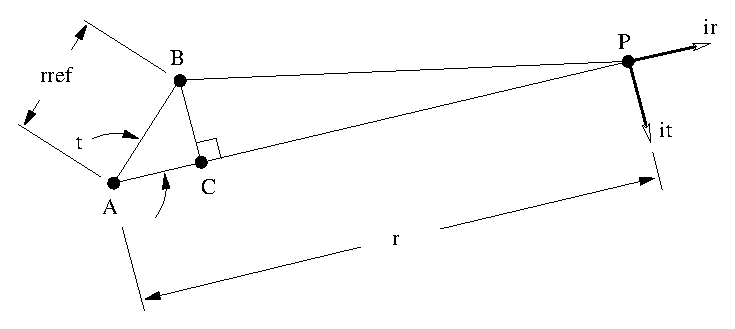
\includegraphics[width=4.0\lengthfigure]{dipoleplane.eps}
\caption{Plane composed of the point where the magnetic field is measured (point ${\vec{P}}$)
         and two points on the dipole axis of symmetry (points $\vec{{A}}$ and ${\vec{B}}$).}
\label{fig:dipoleplane}
\end{figure}
%
and $\vec{i}_\theta$ by normalizing
the vector joining point {$\vec{B}$} to point {$\vec{C}$} (see Fig.\ \ref{fig:dipoleplane}).
%
\begin{equation}
\vec{i}_\theta=\frac{\vec{C}-\vec{B}}{|\vec{C}-\vec{B}|}
\end{equation}
%
where the point $\vec{C}$ corresponds to:
%
\begin{equation}
\vec{C}=r_{\rm ref} \cos \left( \theta \right) \vec{i}_r + \vec{A}
\end{equation}
%
In the above, the angle $\theta$ can be found from the law of the cosines, i.e.
%
\begin{equation}
     \cos \left( \theta \right)=
       \frac{-|\vec{B}-\vec{P}|^2 + |\vec{A}-\vec{P}|^2 + r_{\rm ref}^2}{2 r_{\rm ref}|\vec{A}-\vec{P}|}
\end{equation}
%


\section{Electro Motive Force (EMF)}

The Electro Motive Force (EMF) corresponds to the voltage difference between two electrodes that originate from an external circuit. This voltage difference can sometimes be readily specified on the electrodes within the computational without modeling the external circuit. However, there are some cases where this can not be done. For instance, when there are more than 2 electrodes within one computational domain, the voltage can only be specified a priori on the first two electrodes and must be computed by the flow solver on the remaining electrodes by solving the external circuit. Another problem that requires solving the external circuit is when there is a strong coupling between the plasma and the neutrals leading to a ``runaway'' situation should the voltage difference on the electrodes be fixed. Then, it is necessary to model the external circuit and to limit the voltage difference should too much current (and hence power) flow out of the electrodes. Batteries or other external circuits often have this current limit builtin to prevent damage to the power source. And if they don't, then the current will be limited anyway by some physical process taking place within the power source. Thus, we wish here model such a current limitation within the external circuit.   

For this purpose, consider current flowing through the external governed by Ohm's law as follows:
%
\begin{equation}
 \vec{J}=\sigma (\vec{E} - \vec{E}_{\rm MF})
\end{equation}
%
where $\vec{E}_{\rm MF}$ is the electromotive force vector in V/m that is set by the user (and is not altered by the flow of current), $\vec{E}$ is the electric field vector in V/m that is determined from the potential equation, $\sigma$ is the conductivity of the circuit, and $\vec{J}$ is the current density in A/m$^2$. The power per unit volume deposited to the computational domain corresponds to:
%
\begin{equation}
 {\cal P}=(\vec{E} - \vec{E}_{\rm MF})\cdot \vec{J}
\end{equation}
%  
Substitute the current density from Ohm's law in the latter:
%
\begin{equation}
 {\cal P}=\sigma (\vec{E} - \vec{E}_{\rm MF})\cdot  (\vec{E} - \vec{E}_{\rm MF})
\end{equation}
%  
Now we wish to limit the electro motive force such that the power deposited does not exceed a certain value ${\cal P}_{\rm max}$:
%
\begin{equation}
    (\vec{E} - \psi\vec{E}_{\rm MF})^2 \leq \frac{{\cal P}_{\rm max}}{\sigma}
\end{equation}
% 
where $\psi$ is a limiter function that lies in the range $0\leq \psi \leq 1$. After expanding some terms, we get:
%
\begin{equation}
 \psi^2 \vec{E}_{\rm MF}^2 + \vec{E}^2 - 2 \psi (\vec{E}_{\rm MF}\cdot \vec{E} ) \leq \frac{{\cal P}_{\rm max}}{\sigma}
\end{equation}
% 
We can find the roots of $\psi$ by writing the latter in quadratic form:
%
\begin{equation}
  a \psi^2 + b \phi +c =0
\end{equation}
%
with
%
\begin{align}
  a&= \vec{E}_{\rm MF}^2 \alb
  b&= -2 (\vec{E}_{\rm MF} \cdot \vec{E}) \alb
  c&= \vec{E}^2 - \frac{{\cal P}_{\rm max}}{\sigma}
\end{align}
%
This yields the following roots for $\psi$:
%
\begin{equation}
  \psi=\frac{-b \pm \sqrt{b^2-4ac}}{2a}
\end{equation}
%
Should there be no real root (i.e., if $b^2-4ac<0$) then $\psi$ is set to 0. 


\section{Charge Accumulation on Dielectrics}

\subsection{1D Exact Solution (from Raizer)}

We can find the potential on the dielectric surfaces due to charging following the approach outlined in Ref.\ \cite{tvt:1989:raizer}.

For his purpose, consider a left electrode followed by a plasma of length $L_{\rm p}$ followed by a dielectric of length $L_{\rm d}$ and followed by a right electrode. Define $\Delta \phi_{\rm e}$ as the potential difference between the right and the left electrode, $\Delta \phi_{\rm p}$ as the potential difference within the plasma, and $\Delta \phi_{\rm d}$ as the potential difference within the dielectric. Thus we can say:
%
\begin{equation}
\Delta \phi_{\rm e} = \Delta \phi_{\rm p}+ \Delta \phi_{\rm d}
\end{equation}
% 
We can take the derivative with respect to time of all terms:
%
\begin{equation}
\frac{d}{d t}\Delta \phi_{\rm e} = \frac{d}{d t}\Delta \phi_{\rm p}+ \frac{d}{d t}\Delta \phi_{\rm d}
\label{eqn:ddtDeltaphi}
\end{equation}
% 
Now, from the definition of the capacitance, we can say:
%
\begin{equation}
  C_{\rm d} \frac{\partial}{\partial t} V_{\rm d} = I
\end{equation}
%
where $C_{\rm d}$ is the capacitance of the dielectric, and where $V_{\rm d}$ is the voltage drop within the capacitor, and $I$ is the current (in Amps) flowing in the dielectric. However, by convention the voltage drop within a circuit element is taken as the difference between the left and the right voltages. Thus:
%
\begin{equation}
 V_{\rm d} = -\Delta \phi_{\rm d}
\end{equation}
%
Thus:
%
\begin{equation}
 - C_{\rm d} \frac{\partial}{\partial t} \Delta \phi_{\rm d} = I
\end{equation}
%
 Isolate $\frac{\partial}{\partial t} \Delta \phi_{\rm d}$:
%
\begin{equation}
   \frac{\partial}{\partial t} \Delta \phi_{\rm d} = -\frac{I}{C_{\rm d}}
\end{equation}
%
Substitute the latter in Eq.\ (\ref{eqn:ddtDeltaphi}):
%
\begin{equation}
\frac{d}{d t}\Delta \phi_{\rm e} = \frac{d}{d t}\Delta \phi_{\rm p}- \frac{I}{C_{\rm d}}
\label{eqn:ddtDeltaphie}
\end{equation}
% 
Now we need an expression for the current $I$ which can be obtained noting that the current (including displacement current) at any time is uniform throughout the system:
%
\begin{equation}
  I(t)=A_{\rm cs} J + \underbrace{A_{\rm cs} \epsilon_0 \frac{\partial E}{\partial t}}_{\begin{minipage}{0.1\textwidth}\footnotesize displacement current \end{minipage}}
\end{equation}
%
where $E$ is the electric field, $A_{\rm cs}$ the cross sectional area of the plasma (perpendicular to the motion of the charges), $\epsilon_0$ the permittivity of free space, and where $J$ is the current density due to the motion of the charges:
%
\begin{equation}
  J=\sum_{k=1}^\ns C_k N_k V_k
\end{equation}
%
with $C_k$ the charge of species $k$, $N_k$ the number density of species $k$, and $V_k$ the velocity of species $k$ along $x$ including drift, diffusion, and temperature gradients (see Eq.\ (\ref{eqn:V})). Note that the sum of the displacement current and the current due to the motion of the charges  is only function of time, not of space. 

Now integrate the total current through the plasma:
%
\begin{equation}
  \int_{x=0}^{x=L_{\rm p}} I dx=\int_{x=0}^{x=L_{\rm p}} A_{\rm cs} J dx + \epsilon_0 A_{\rm cs} \int_{x=0}^{x=L_{\rm p}} \frac{\partial E}{\partial t}  dx
\end{equation}
%
But $I$ only depends on time, and does not depend on space. Thus:
%
\begin{equation}
  I L_{\rm p}=\int_{x=0}^{x=L_{\rm p}} A_{\rm cs} J dx + \epsilon_0 A_{\rm cs} \int_{x=0}^{x=L_{\rm p}} \frac{\partial E}{\partial t}  dx
\end{equation}
%
Note that the integral of a derivative is the derivative of an integral:
%
\begin{equation}
  I L_{\rm p}=\int_{x=0}^{x=L_{\rm p}} A_{\rm cs} J dx + \epsilon_0 A_{\rm cs} \frac{d }{d t} \int_{x=0}^{x=L_{\rm p}} E  dx
\end{equation}
%
Note that the electric field is the negative of the gradient of the potential:
%
\begin{equation}
  I L_{\rm p}=\int_{x=0}^{x=L_{\rm p}} A_{\rm cs} J dx + \epsilon_0 A_{\rm cs} \frac{d }{d t} \int_{x=0}^{x=L_{\rm p}} -\frac{\partial \phi}{\partial x}  dx
\end{equation}
%
Thus:
%
\begin{equation}
  I L_{\rm p}=\int_{x=0}^{x=L_{\rm p}} A_{\rm cs} J dx - \epsilon_0 A_{\rm cs} \frac{d }{d t} \int_{x=0}^{x=L_{\rm p}} d \phi
\end{equation}
%
This yields:
%
\begin{equation}
  I L_{\rm p}=\int_{x=0}^{x=L_{\rm p}} A_{\rm cs} J dx - \epsilon_0 A_{\rm cs} \frac{d }{d t}  \Delta \phi_{\rm p}
\end{equation}
%
Isolate $I$ in the latter:
%
\begin{equation}
  I =\frac{1}{L_{\rm p}}\int_{x=0}^{x=L_{\rm p}} A_{\rm cs} J dx - \frac{\epsilon_0 A_{\rm cs}}{L_{\rm p}} \frac{d }{d t}  \Delta \phi_{\rm p}
\label{eqn:I}
\end{equation}
%
Substitute $I$ from Eq.\ (\ref{eqn:I}) in Eq.\ (\ref{eqn:ddtDeltaphie}):
%
\begin{equation}
\frac{d}{d t}\Delta \phi_{\rm e} = \frac{d}{d t}\Delta \phi_{\rm p}- \left(\frac{1}{C_{\rm d} L_{\rm p}}\int_{x=0}^{x=L_{\rm p}} A_{\rm cs} J dx - \frac{\epsilon_0 A_{\rm cs}}{C_{\rm d} L_{\rm p}} \frac{d }{d t}  \Delta \phi_{\rm p} \right)
\end{equation}
% 
Regroup:
%
\begin{equation}
\frac{d}{d t}\Delta \phi_{\rm e} = \left(1+\frac{\epsilon_0 A_{\rm cs}}{C_{\rm d} L_{\rm p}} \right)\frac{d}{d t}\Delta \phi_{\rm p}- \frac{1}{C_{\rm d} L_{\rm p}}\int_{x=0}^{x=L_{\rm p}} A_{\rm cs} J dx  
\end{equation}
% 
We can express the dielectric capacitance as:
%
\begin{equation}
 C_{\rm d}=\epsilon_r \epsilon_0 \frac{A_{\rm cs}}{L_{\rm d}}
\end{equation}
%
where $\epsilon_0$ is the permittivity of free space ($\rm 8.85419 \times 10^{-12} \, m^{-3} \, kg^{-1} \, s^4 \, A^2$), $\epsilon_r$ is the relative static permittivity (a.k.a. dielectric constant), $A_{\rm cs}$ is the cross-sectional area of the dielectric perpendicular to the current in $\rm m^2$, and $L_{\rm d}$ is the length of the dielectric in the direction of the current in meters. The following would yield a dielectric capacitance in Farad (same units as $\rm A \, s \, V^{-1}$). Note that a kg can be expressed in units of $\rm s^3 \, V \, A \, m^{-2}$ and that $\epsilon_0$ can be expressed in units of $\rm s \, A \, m^{-1} \, V^{-1}$. Substituting the latter in the former, we obtain:
%
\begin{equation}
\frac{d}{d t}\Delta \phi_{\rm e} = \left(1+\frac{ L_{\rm d}}{\epsilon_r  L_{\rm p}} \right)\frac{d}{d t}\Delta \phi_{\rm p}- \frac{L_{\rm d}}{\epsilon_r \epsilon_0  L_{\rm p}}\int_{x=0}^{x=L_{\rm p}}  J dx  
\end{equation}
% 
Now, isolate the integral of the current density:
%
\begin{equation}
\frameeqn{
 \int_{x=0}^{x=L_{\rm p}}  J dx  
=
 \left(\frac{\epsilon_r \epsilon_0  L_{\rm p}}{L_{\rm d}} +\epsilon_0   \right)\frac{d}{d t}\Delta \phi_{\rm p} 
-\left( \frac{\epsilon_r \epsilon_0  L_{\rm p}}{L_{\rm d}} \right)\frac{d}{d t}\Delta \phi_{\rm e} 
}
\end{equation}
% 
The latter can be used as a means of code validation: knowing the potential difference on the electrodes $\Delta \phi_{\rm e}$ and measuring the potential difference on the plasma $\Delta \phi_{\rm p}$ within the numerical results, the latter equation yields an analytical expression for the integral of the current density which can be compared with its numerically-obtained counterpart.    


\subsection{1D Exact Solution (from Ohm's law)}

After substituting the displacement current outlined in Eq.\ (\ref{eqn:Jdisplacement}) into the total current within Eq.\ (\ref{eqn:Jtotal}), we obtain:
%
\begin{equation}
 J^{\rm t} =
  -~\epsilon_0 \epsilon_r \frac{\partial (\partial_t \phi)}{\partial x}
+J
\end{equation}
%
Multiply both sides by $dx$ and integrate through the plasma from $x=0$ till $x=L_{\rm p}$ with $L_{\rm p}$ the length of the plasma:
%
\begin{equation}
\int_0^{L_{\rm p}} J^{\rm t} dx =
  - \int_0^{L_{\rm p}} \epsilon_0 \epsilon_r d (\partial_t \phi)
+\int_0^{L_{\rm p}} J dx
\end{equation}
%
Consider a plasma with $\epsilon_r$ equal to 1:
%
\begin{equation}
\int_0^{L_{\rm p}} J^{\rm t} dx =
  - \epsilon_0  \int_0^{L_{\rm p}}  d (\partial_t \phi)
+\int_0^{L_{\rm p}} J dx
\end{equation}
%
But the total current is constant through the plasma:
%
\begin{equation}
J^{\rm t} L_{\rm p}=
  - \epsilon_0  \int_0^{L_{\rm p}}  d (\partial_t \phi)
+\int_0^{L_{\rm p}} J dx
\end{equation}
%
Integrate the first integral on the RHS:
%
\begin{equation}
J^{\rm t} L_{\rm p}=
  - \epsilon_0  \left( (\partial_t \phi)_{x=L_{\rm p}} - (\partial_t \phi)_{x=0} \right)
+\int_0^{L_{\rm p}} J dx
\end{equation}
%
or,
%
\begin{equation}
J^{\rm t} L_{\rm p}=
  - \epsilon_0  \partial_t (\phi_{x=L_{\rm p}} - \phi_{x=0}) 
+\int_0^{L_{\rm p}} J dx
\end{equation}
%
or,
%
\begin{equation}
J^{\rm t} L_{\rm p}=
  - \epsilon_0  \partial_t \Delta \phi_{\rm p} 
+\int_0^{L_{\rm p}} J dx
\label{eqn:JtLp1}
\end{equation}
%
with $\Delta \phi_{\rm p}$ the potential difference through the plasma. 

Now repeat the latter steps but within the dielectric. Start with the total current and note that the conduction current $J$ is zero within the dielectric:
%
\begin{equation}
 J^{\rm t} =
  -~\epsilon_0 \epsilon_r \frac{\partial (\partial_t \phi)}{\partial x}
\end{equation}
%
Multiply both sides by $dx$ and integrate through the dielectric from $x=0$ till $x=L_{\rm d}$ with $L_{\rm d}$ the length of the dielectric:
%
\begin{equation}
 J^{\rm t} L_{\rm d} =
  -~\epsilon_0 \epsilon_r \partial_t \Delta \phi_{\rm d}
\end{equation}
%
with $L_{\rm d}$ the length of the dielectric and $\Delta \phi_{\rm d}$ the potential difference across the dielectric. Multiply both sides by $L_{\rm p}/L_{\rm d}$:
%
\begin{equation}
 J^{\rm t} L_{\rm p} =
  -~\epsilon_0 \epsilon_r \frac{L_{\rm p}}{L_{\rm d}} \partial_t \Delta \phi_{\rm d} 
\label{eqn:JtLp2}
\end{equation}
%
Substitute the latter in Eq.\ (\ref{eqn:JtLp1}).
%
\begin{equation}
  -~\epsilon_0 \epsilon_r \frac{L_{\rm p}}{L_{\rm d}} \partial_t \Delta \phi_{\rm d} 
=
  - \epsilon_0  \partial_t \Delta \phi_{\rm p} 
+\int_0^{L_{\rm p}} J dx
\end{equation}
%
Isolate the current integral:
%
\begin{equation}
\frameeqn{
\int_0^{L_{\rm p}} J dx
=
  - \epsilon_0 \epsilon_r \frac{L_{\rm p}}{L_{\rm d}} \partial_t \Delta \phi_{\rm d} 
  + \epsilon_0  \partial_t \Delta \phi_{\rm p} 
}
\end{equation}
%
Now consider a system composed of an electrode, followed by a plasma of length $L_{\rm p}$, followed by a dielectric of length $L_{\rm d}$, followed by another electrode. The potential difference between the two electrodes, $\Delta \phi_{\rm e}$, can be written as: 
%
\begin{equation}
\Delta \phi_{\rm e}=\Delta \phi_{\rm p} + \Delta \phi_{\rm d}
\end{equation}
%
Isolate $\Delta \phi_{\rm d}$ in the latter and substitute in the former:
%
\begin{equation}
\frameeqn{
\int_0^{L_{\rm p}} J dx
=
    \epsilon_0 \left(1+\epsilon_r \frac{L_{\rm p}}{L_{\rm d}} \right) \partial_t \Delta \phi_{\rm p} 
  - \epsilon_0 \epsilon_r \frac{L_{\rm p}}{L_{\rm d}} \partial_t \Delta \phi_{\rm e} 
}
\end{equation}
%



\subsection{Surface Charge Density for Gauss-based Potential Equation Solver}

Consider a plasma bounded by a dielectric surface. The rate of change of the surface charge density corresponds to the current density coming towards it:
%
\begin{equation}
  \frac{\partial \sigma_{\rm s}}{\partial t} = -\vec{J}_{\chi}  
\label{eqn:dsigmasdt}
\end{equation}
%
with $\chi$ a coordinate perpendicular to the surface and that points from the surface towards the plasma and where 
 $\vec{J}_\chi$ is the component of the current density vector in the direction of $\chi$ (in units of Amps per square meter), and where $\sigma_{\rm s}$ is the surface charge density in Coulombs per square meter. When the plasma is at steady-state, $\vec{J}_\chi$ becomes zero but $\sigma_{\rm s}$ does not become zero. That is, the surface charge will adjust such that it creates an electric field just strong enough for the current perpendicular to the dielectric to vanish. 

Recall Gauss's law:
%
\begin{equation}
  \frac{\partial }{\partial \chi} \epsilon_0 \vec{E}_\chi = \underbrace{\sigma_{\rm s} A_{\rm cs}}_{\begin{minipage}{0.1\textwidth}\footnotesize\flushleft net charge on surface\end{minipage}} \underbrace{\frac{1}{A_{\rm cs} \Delta \chi}}_{\begin{minipage}{0.075\textwidth}\footnotesize\flushleft per unit volume\end{minipage}} 
\end{equation}
% 
with $\vec{E}_\chi$ the electric field component in the direction of $\chi$ and $\epsilon_0$ the permittivity of free space. Note that the space charge is assumed to be located out of the dielectric within the plasma, hence why the dielectric constant is not included within Gauss's law.

Then, we can multiply both sides by $d \chi$ and obtain:
%
\begin{equation}
  d (\epsilon_0 \vec{E}_\chi) = \frac{\sigma_{\rm s} A_{\rm cs}}{A_{\rm cs} \Delta \chi} d \chi 
\end{equation}
% 
Integrate from $\chi=0$ to $\chi=\Delta \chi$ with $\Delta \chi$ being the thickness of the plasma region close to the dielectric where the charges build up:
%
\begin{equation}
 \int_{\chi=0}^{\chi=\Delta \chi}  d(\epsilon_0 \vec{E}_\chi) = \int_{\chi=0}^{\chi=\Delta \chi} \frac{\sigma_{\rm s} A_{\rm cs}}{A_{\rm cs} \Delta \chi} d \chi 
\end{equation}
% 
Assume that the surface charge $\sigma_{\rm s}$ is constant from $\chi=0$ to $\chi=\Delta \chi$. This yields:
%
\begin{equation}
 \epsilon_0 \left( \left(\vec{E}_\chi\right)_{\chi=\Delta \chi} 
                 - \left(\vec{E}_\chi\right)_{\chi=0}\right)
  = 
 \sigma_{\rm s}  
\end{equation}
% 
Or, in short form:
%
\begin{equation}
  \Delta \vec{E}_\chi
  = 
 \frac{\sigma_{\rm s}}{\epsilon_0}  
\label{eqn:deltaE}
\end{equation}
% 
where $\Delta \vec{E}_\chi$ is the electric field that must be added to the existing electric field at the dielectric surfaces due to charge accumulation.  


\subsection{Characteristic Time Scale For Surface Charging}

Isolate $\sigma_{\rm s}$ in Eq.\ (\ref{eqn:deltaE}) and substitute in Eq.\ (\ref{eqn:dsigmasdt}):
%
\begin{equation}
  \frac{\partial}{\partial t} \epsilon_0 \Delta \vec{E}_\chi = -\vec{J}_{\chi}  
\end{equation}
%
At the surface, we can say that $\vec{J}_\chi=\sigma \vec{E}_\chi$ with $\sigma$ the conductivity of the plasma at the surface:
%
\begin{equation}
  \frac{\partial}{\partial t} \epsilon_0 \Delta \vec{E}_\chi = -\sigma \vec{E}_\chi  
\end{equation}
%
Thus, the characteristic time step associated with surface charging, $dt \approx \Delta t$, can be taken as:
%
\begin{equation}
    \Delta t \sim  \frac{ \epsilon_0}{\sigma} \left| \frac{\Delta \vec{E}_\chi}{\vec{E}_\chi}\right| 
\end{equation}
%
For the surface charge to reach an equilibrium, $|\Delta \vec{E}_\chi| \sim |\vec{E}_\chi|$. Thus:
%
\begin{equation}
\frameeqn{
    \Delta t \sim  \frac{ \epsilon_0}{\sigma}  
}
\end{equation}
%


\section{Recast of $\vec{E}\cdot \vec{J}$}

Start from the definition of the Joule heating outlined in the Appendix of Ref.\ \cite{aiaa:2016:parent}:
%
\begin{equation}
 Q_{\rm J} = \underbrace{  \sum_{r=1}^{n_{\rm cs}} \left( C_r N_r \left( \vec{E}+\vec{V}^r \times\vec{B}\right)  - \vec{\nabla} P_r \right)\cdot \vec{V}^r}_{\textrm{\begin{minipage}{3cm}\flushleft \footnotesize work done on the charged species in the lab frame\end{minipage}}} 
- \underbrace{\left(\rho_{\rm c} \vec{E} + \vec{J}\times\vec{B} -\sum_{r=1}^{n_{\rm cs}} \vec{\nabla} P_r \right)\cdot \vec{V}^{\rm n}}_{\textrm{\begin{minipage}{4cm}\flushleft \footnotesize work done by the charged species on the neutrals in the lab frame\end{minipage}}}
\end{equation}
%
where $n_{\rm cs}$ is the number of charged species. But $(\vec{V}^r \times\vec{B})\cdot \vec{V}^r=0$. Thus:
%
\begin{equation}
 Q_{\rm J} =   \sum_{r=1}^{n_{\rm cs}} \left( C_r N_r  \vec{E}  - \vec{\nabla} P_r \right)\cdot \vec{V}^r 
- \left(\rho_{\rm c} \vec{E} + \vec{J}\times\vec{B} -\sum_{r=1}^{n_{\rm cs}} \vec{\nabla} P_r \right)\cdot \vec{V}^{\rm n}
\end{equation}
%
Rewrite as:
%
\begin{equation}
 Q_{\rm J} =   \sum_{r=1}^{n_{\rm cs}} \left( C_r N_r  \vec{E}   \right)\cdot \vec{V}^r 
-  \sum_{r=1}^{n_{\rm cs}} \vec{\nabla} P_r \cdot \vec{V}^r 
- \left(\rho_{\rm c} \vec{E} + \vec{J}\times\vec{B} -\sum_{r=1}^{n_{\rm cs}} \vec{\nabla} P_r \right)\cdot \vec{V}^{\rm n}
\end{equation}
%
or,
%
\begin{equation}
 Q_{\rm J} =   \sum_{r=1}^{n_{\rm cs}} \left( C_r N_r  \vec{E}   \right)\cdot \vec{V}^r 
+  \sum_{r=1}^{n_{\rm cs}} \vec{\nabla} P_r \cdot \left(\vec{V}^{\rm n}-\vec{V}^r\right) 
- \left(\rho_{\rm c} \vec{E} + \vec{J}\times\vec{B} \right)\cdot \vec{V}^{\rm n}
\end{equation}
%
After substituting the current density $\vec{J}$ we obtain: 
%
\begin{equation}
 Q_{\rm J} =     \vec{E} \cdot \vec{J} 
+  \sum_{r=1}^{n_{\rm cs}} \vec{\nabla} P_r \cdot \left(\vec{V}^{\rm n}-\vec{V}^r\right) 
- \left(\rho_{\rm c} \vec{E} + \vec{J}\times\vec{B} \right)\cdot \vec{V}^{\rm n}
\end{equation}
%
Isolate $\vec{E}\cdot\vec{J}$:
%
\begin{equation}
\vec{E} \cdot \vec{J}
=
 \left(\rho_{\rm c} \vec{E} + \vec{J}\times\vec{B} \right)\cdot \vec{V}^{\rm n}
+ Q_{\rm J} 
+  \sum_{r=1}^{n_{\rm cs}} \vec{\nabla} P_r \cdot \left(\vec{V}^r-\vec{V}^{\rm n}\right) 
\end{equation}
%
At the differential level, the RHS is exactly equal to the LHS. However, at the discrete level, the LHS could differ from the RHS by a large amount. This can then lead to negative temperatures within the solution because the gas temperature is determined from the subtraction of $e_{\rm t}$ and $e_{\rm v}$ with the latter being function of $Q_{\rm J}$. Thus, to prevent negative gas temperatures, it is recommended to substitute $\vec{E}\cdot\vec{J}$ by $\left(\rho_{\rm c} \vec{E} + \vec{J}\times\vec{B} \right)\cdot \vec{V}^{\rm n}
+ Q_{\rm J} +  \sum_{r=1}^{n_{\rm cs}} \vec{\nabla} P_r \cdot \left(\vec{V}^r-\vec{V}^{\rm n}\right)$ within the total energy equation.


 

  \bibliographystyle{warpdoc}
  \bibliography{all}


\end{document}




